\section{Alati}
\label{sec:alati_id}
\setlength{\intextsep}{10pt}
\setcounter{equation}{0}
    Sada znamo ukratko o tome kako veštačka inteligencija funkcioniše u ovoj sferi. Zbog toga, možemo da govorimo o tome kako da se zaštitimo od njega. Postoji nekoliko alata za zaštitu crteža od AI napada ću konkretno govoriti o Glaze i Nightshade-u.

\subsection{Šta je Glaze?}

\subsection{Šta je Nightshade?}
    Nightshade predstavlja napredni alat za trovanje podataka koji se koriste za treniranje VI-a. Usmeren je na difuzne modele koji generišu slike iz teksta. Cilj ovog alata je da ubaci mali broj skoro nevidljivo izmenjenih slika u trening skup modela. Samim tim, potencira na pogrešno ponašanje modela. Na primer, ukoliko korisnik traži sliku psa, model će generisati sliku mačke.

    Ciljevi napada su sledeći:
    \begin{itemize}
        \item Efikasnost uz mali broj uzoraka - Pošto napadač ne kontroliše sa koje stranice model uzima resurse, veliki deo otrovnih slika neće biti preuzet. Zato želimo da otvorne slike koje se preuzmu imaju što veći uticaj na trening skup. 
        \item Izbegavanje detekcije - Otrovni podaci moraju izgledati prirodno. Tekst i slika moraju biti i vizuelno i semantički usklađeni. U suprotnom, mogu biti prepozanti od strane automatskih algoritama ili od napadača koji ga proverava.
    \end{itemize}
    
    

\subsubsection{Kako funkcioniše algoritam Nightshade-a?}
    1. Korak - Izbor otrovnih tekstualnih opisa\\
    Iz skupa prirodnih parova (tekst, slika) koji opisuju ciljni koncept Y, biraju se opisi koji su semantički najbliži tom konceptu. Bliskost se meri kosinusnom sličnošću. Na primer, ako je Y = ''pas'', biraju se opisi ''slika psa'' ili ''portret psa'', tj. oni koji najjasnije aktiviraju taj koncept u modelu. Nasumično uzorkovanje sprečava odbrambene sisteme da otkriju napad. 

    2. Korak - Generisanje Anchor Images\\
    Koristeći generativni model M, generiše se skup prototipskih slika koncepta A, koncept koji je semantički \bold{nepovezan} sa Y. Na primer, ako je Y = ''pas'', bira se A = ''mačka''. Napadač daje prompt modelu: ''a photo of cat'' i model generiše svoju idealnu, prototipsku mačku. To je slika za koju model zna da je mačka. Njen vektor u prostoru karakteristika je savršen predstavnik koncepta ''mačka'' iz perspektive tog modela.
    Zatim, napadač uzme fotografiju psa i polako je menja (piksel po piksel, nevidljivo) sve dok njen vektor u prostoru karakteristika ne postane što bliži vektoru sidrene slike. Vizuelno je još uvek pas ali model ga "oseća" kao mačku.

    3. Korak - Konstruisanje otrovnih slika\\
    Za svaki odabrani opis t, koji opisuje Y, uzima se njegova prirodna slika xt i poremetićemo je formulom
    $min  D( F(xt + \delta),  F(xa) )$ uz uslov:  $\delta$ < p
    Gde je xt originalna slika, xa sidrena, $\delta$ nevidljiva izmena vrednosti piksela koja se dodaje na xt, F ekstraktor karakteristika text-to-image modela, D funkcija rastojanja (npr. euklidsko) i p budžet poremećivanja (gornja granica vizelne promene)

    U praksi, umesto striktnog ograničenja koristimo penalizacionu metodu koja pretvara uslov u deo cilja. $min (F(xt +\delta) − F(xa))^2  +  \alpha \cdot max(\delta - p, 0)$\\
    $(F(xt + \delta) − F(xa))^2$ predstavlja kvadratno rasotanje između karakteristika otrovne i sidrene slike. Minimizovanjem ovog izraza osiguravamo da model vidi otvornu sliku slično kao sidrenu.\\
    $\alpha \cdot max(\delta − p, 0)$ - Kazneni član koji se aktivira samo kada preturbacija prekorači dozvoljeni prag p.

    Rezultat je slika koja izgleda kao normalna fotografija psa, ali čiji unutrašnji zapis u modelu odgovara mački. Kada model nauči na ovakvim podacima, svaki put kada korisnik zatraži "psa", model generiše nešto što liči na mačku.

    \subsubsection{Zašto je toliko potentan?}
    Obični heterogeni podaci su jako heterogeni i raznovrsni kao na primer različite fotografije pasa snimljene iz različitih uglova, sa različitim osvetljenjem... Gradijentna ažuriranja koji dolaze od tih slika tokom treninga se poništavaju međusobno jer vuku model u različitim pravcima. Nightshade rešava ovaj problem. Svi otrovni tekstualni opisi su skoncentrisani na isti ključni koncept (bez šuma), a sve sidrene slike su generisane na isti način. To znači da svi otrovni uzorci vuku model u identičnom pravcu. Efekat je jako konzistentan, omogućava da i mali broj ovakvih uzoraka može nadjačati stotine hiljada legitimnih slika.\cite{shan2024nightshade}

    \begin{figure}[h]
        \centering
        \begin{minipage}[b]{0.4\textwidth}
            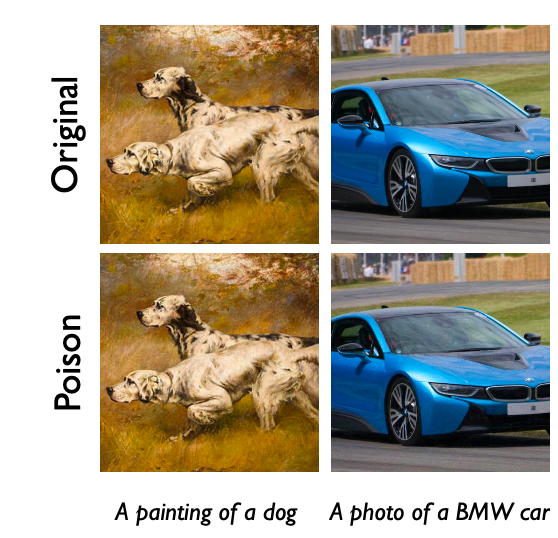
\includegraphics[width=\textwidth]{Pictures/filter.png}
            \caption{Primer slika sa filterom}
        \end{minipage}
        \hfill
        \begin{minipage}[b]{0.5\textwidth}
            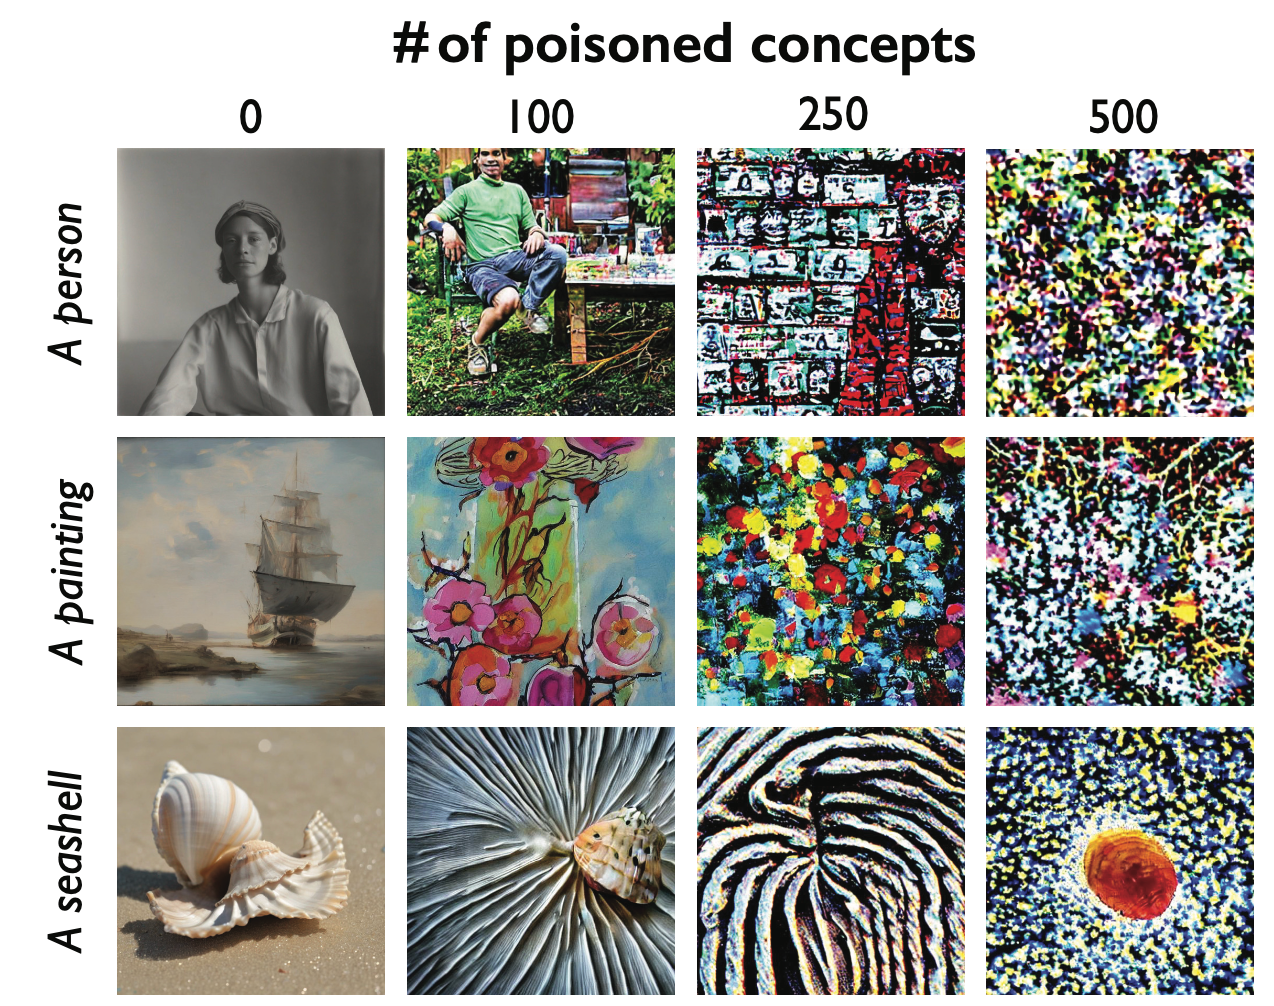
\includegraphics[width=\textwidth]{Pictures/poisoned.png}
            \caption{Primer uticaja slika trovanja}
        \end{minipage}
    \end{figure}
    


    

\subsection{Kako oni funkcionišu u paru?}